\documentclass{beamer}
\usetheme{Warsaw}
\useinnertheme{circles}
\useoutertheme[subsection=false]{smoothbars}
\usepackage[utf8x]{inputenc}
\usepackage[czech]{babel}
\usepackage[T1]{fontenc}
\usepackage{listings}
\usepackage{tikz}

\begin{document}

\AtBeginSection[]
{
  \begin{frame}
    \frametitle{Outline}
    \tableofcontents[currentsection]
  \end{frame}
}

\title{Open source programování}
\subtitle{Otevřené prostředí a hračky}
\author{Petr Baudiš $\langle${\tt pasky@ucw.cz}$\rangle$}
\institute{MFF UK 2011\\
	\vskip 1ex
	\pgfdeclareimage[height=4ex]{ccbysa}{by-sa.pdf}
	\pgfuseimage{ccbysa}
}
\date{}
\frame{\titlepage}

\section{Úvod}

\subsection{}
\begin{frame}{O čem dnes}
\begin{itemize}
\item Systémové prostředí: Otevřený desktop
\item Programátorské prostředí: Knihovny, \\ dokumentace a~skriptování
\item Otevřený hardware: Opět úžasný nový svět
\end{itemize}
\end{frame}


\section{Systémové prostředí}

\subsection{}
\begin{frame}{Jádro systému}
\begin{itemize}
\item POSIXové API, systém plně kompatibilní s UNIXem
\item Pevné ABI k userlandu, nestálé ABI v rámci jádra
\item Monolitický ale modulární, objektové C
\item Portabilní: Atmel AVR32 $\to$ IBM BlueGene
\pause
\vskip 3ex
\item Rozhraní: Systémová volání, speciální soubory, \\ speciální souborové systémy, callbacky
\end{itemize}
\end{frame}

\subsection{}
\begin{frame}{Základní userspace}
\begin{itemize}
\item util-linux --- nástroje specifické pro Linux (např. {\tt mount})
\item GNU coreutils --- základní UNIXové příkazy
\item GNU libc (glibc) --- Cčkový runtime, API k systémovým voláním, dynamický linker
\item GNU toolchain (gcc, binutils, make)
\item Alternativy: Busybox, uClibc
\end{itemize}
\end{frame}

\subsection{}
\begin{frame}{Koordinace služeb}
\begin{itemize}
\item sysvinit / upstart + inetd, systemd
\item dbus --- message passing sběrnice
\pause
\vskip 3ex
\item {\bf Bootování:} BIOS (coreboot), GRUB, vmlinuz
\item (initrd), připojení / filesystému (read-only)
\item /sbin/init
\item Základní služby: udev, připojení souborových systémů, síť, \dots
\item Runlevel: logování, síťové služby, login manažer a obsluha tty
\end{itemize}
\end{frame}

\subsection{}
\begin{frame}{Rozhraní ``jádra''}
\begin{itemize}
\item udev --- údržba /dev souborů a spousta dalšího
\item DeviceKit: libudev (/sys), udisks, upower
\item (HAL už je naštěstí mrtev)
\item PolicyKit, ConsoleKit, PackageKit
\item NetworkManager, GStreamer / PulseAudio / ALSA, X~extensions
\end{itemize}
\end{frame}

\subsection{}
\begin{frame}{Desktopové prostředí}
\begin{itemize}
\item X.org (+KMS, DRM, DRI, XI2+XRandR)
\item FreeDesktop.org
\item GNOME, KDE, Xfce, \dots
\item Firefox, SpiderMoneky, jslinux --- a jedeme znovu! ;-)
\end{itemize}
\end{frame}

\subsection{}
\begin{frame}{Skládačka}
\begin{itemize}
\item Naučte se v praxi --- Linux From Scratch!
\item Nebo alespoň Gentoo
\end{itemize}
\end{frame}


\section{Programátorské prostředí}

\subsection{}
\begin{frame}{GNU libc}
\begin{itemize}
\item {\bf glibc} --- C runtime (ne C++), POSIXové API a příbuzní
\item Standardy --- Cx9, POSIX.*, SysV/BSD
\item Částečná koevoluce s libiberty a GNUlib
{\footnotesize \item Charsets a locales, gettext runtime, třídění a vyhledávání, matchování globů a regulárních výrazů, I/O nad streamy i deskriptory, soubory a sockety, terminály, signály a IPC, procesy, job control, syslog, name resolution, matematické funkce, datum a čas, control flow, dynamický linker, proměnné prostředí, charakteristiky systému, kryptografické funkce}
\item Multi-threading (pthreads: NPTL, (mrtvé) LinuxThreads)
\item Zajímavé featurky: I/O (vektorové, asynchronní, mmapové, dyn. alokované, \dots), dočasné soubory, {\tt backtrace()}, NSS, customizace {\tt printf}, rozšíření paměťového alokátoru, obstacks
\item Často GNU rozšíření pro reentrantní verze; \\ {\tt strverscmp()}, hledej {\tt \_GNU\_SOURCE}
\end{itemize}
\end{frame}

\subsection{}
\begin{frame}{Systémové knihovny}
\begin{itemize}
\item libevent
\item libnih
\item GLib
\item libucw
\vskip 3ex
\begin{block}{Terminálové knihovny}
\begin{itemize}
\item Termcap a terminfo
\item GNU Readline
\item NCurses
\item SLang
\end{itemize}
\end{block}
\end{itemize}
\end{frame}

\subsection{}
\begin{frame}{Omalovánkové knihovny}
\begin{itemize}
\item SDL --- ``low-level'' grafika, I/O, zvuk, \dots
\item Cairo --- vektorová grafika, mnoho výstupů
\item GTK --- okénka Cčkově (event a callback)
\item Qt --- okénka C++kově (signal a slot), i non-GUI věci
\end{itemize}
\end{frame}

\subsection{}
\begin{frame}{Dokumentace UNIXových programů}
\begin{itemize}
\item Manuálové stránky (linux-manpages)
\item GNU info (pinfo!)
\item Web $:-($
\item Use the Source, Luke
\end{itemize}
\end{frame}

\subsection{}
\begin{frame}{Generování dokumentace}
\begin{center}
\begin{block}{Docbook}
\begin{itemize}
\item Dokumentace v (rozumném) XML formátu, \\ export do spousty výstupních formátů (HTML, PDF, man, \dots)
\item Preprocesory (asciidoc, markdown, \dots)
\end{itemize}
\end{block}
\begin{block}{Doxygen}
\begin{itemize}
\item Referenční programátorská dokumentace
\item Z komentářů přímo v kódu
\item Automatické cross-reference
\end{itemize}
\end{block}
\end{center}
\end{frame}

\subsection{}
\begin{frame}{Skriptování: Shell}
\begin{itemize}
\item GNU bash, zsh, (dash)
\item GNU coreutils
\item POSIX (aktivní drive; {\tt \$POSIXLY\_CORRECT})
\item Roztodivná rozšíření
\end{itemize}
\end{frame}

\subsection{}
\begin{frame}{Skriptování: Další}
\begin{itemize}
\item Perl: There is more than one way to do it
\item Python: There should be one --- and preferably only one --- obvious way to do it
\item Scheme: Tradiční skriptovací jazyk GNU
\item Tcl: Hordy zombies
\item Lua, CLisp, Ruby, PHP, \dots
\vskip 3ex
\item SWIG: Bindingy C funkcí do různých skriptovacích jazyků
\item Naopak: Problematické, nutno ručně
\vskip 3ex
\item flex a bison --- scanner a parser (generátor C kódu)
\end{itemize}
\end{frame}


\section{Otevřený hardware}

\subsection{}
\begin{frame}{Úžasný nový svět}
\begin{itemize}
\item GNU: Uživatel by měl mít přístup k veškerému software, \\ které používá
\item V dnešní době málokdo používá software pouze \\ ve stolním počítači
\item Mikročipy jsou levné, elektroniku kolem si snadno \\ postaví mnoho lidí
\item Ekonomika technologií se mění na komoditní
\end{itemize}
\end{frame}

\subsection{}
\begin{frame}{Hackerspaces}
\begin{columns}
\begin{column}{3cm}

\includegraphics[width=3cm]{hackerspaces.png}
\vskip 1ex
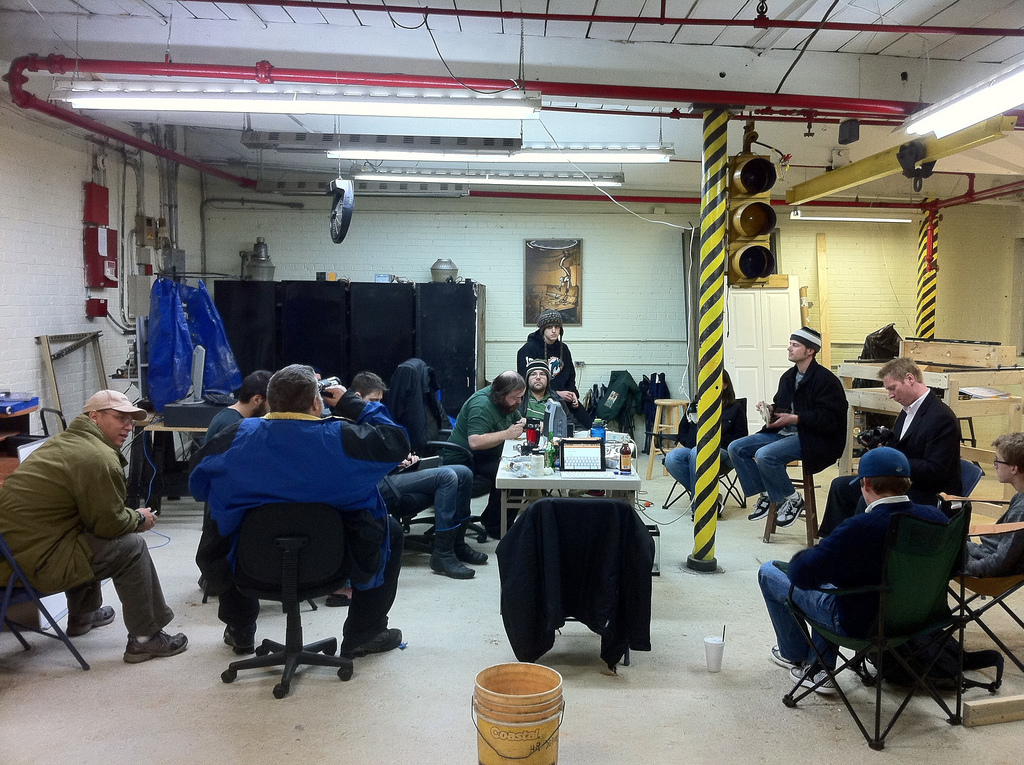
\includegraphics[width=3cm]{Hackerspace_charlotte.jpg}
\vskip 1ex

\includegraphics[width=3cm]{brmlab.pdf}
\vskip 1ex
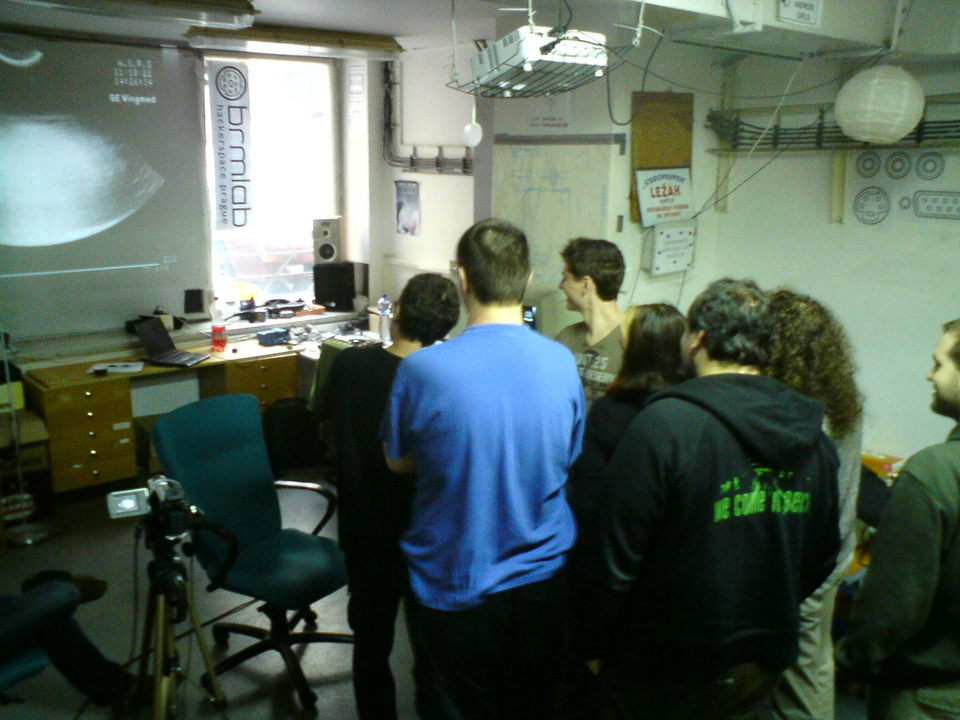
\includegraphics[width=3cm]{brmlab-us.jpeg}
\end{column}
\begin{column}{8cm}
\begin{itemize}
\item Internet umožnil celosvětovou spolupráci programátorů
\item Místní spolupráci zajišťovaly univerzity a~velké společnosti
\item Širší dostupnost technologií $\Rightarrow$ fragmentovaná komunita
\pause
\vskip 3ex
\item {\bf Hackerspace} nebo {\bf makerspace} \\ (Svazarm, radioklub, \dots)
\item Nezávislé, řízené komunitou, \\ provozované hackery
\item ``DIY'', Open Source kultura
\item Kritická masa, sdílení idejí, \\ základna pro větší projekty
\end{itemize}
\end{column}
\end{columns}
\end{frame}

\subsection{}
\begin{frame}{Open Source firmware}
\begin{itemize}
\item Telefony a tablety --- Google Android (Cyanogen Mod), Nokia~Maemo / Meego
\item Wifi routery --- OpenWRT, DD-WRT, \dots
\item Další telefony, MP3 přehrávače, autorádia, \dots
\end{itemize}
\end{frame}

\subsection{}
\begin{frame}{Open Source hardware}
\begin{itemize}
\item Mikrokontrolérová destička Arduino!
\item Počítání v oblečení (wearable computing), \\ světélka a automatizace domácnosti, \\ roboti, quadkoptéry (hackaday.com)
\item DIY Bio: OpenPCR, jednoduché hacky \\ k analýze DNA, OpenEEG
\item OpenMoko aj. open source telefony a PDA; \\ Raspberry Pi
\vskip 3ex
\item Integrované obvody pomocí FPGA (OpenSPARC, etc.)
\item USRP a GNU Radio --- hack the EM spectrum
\vskip 3ex
\item Global Village Construction Kit
\item RepRap / MakerBot --- 3D tisk!
\end{itemize}
\begin{tikzpicture}[remember picture,overlay]
  \node [xshift=-4.25cm,yshift=-4.5cm,above right] at (current page.north east)
    {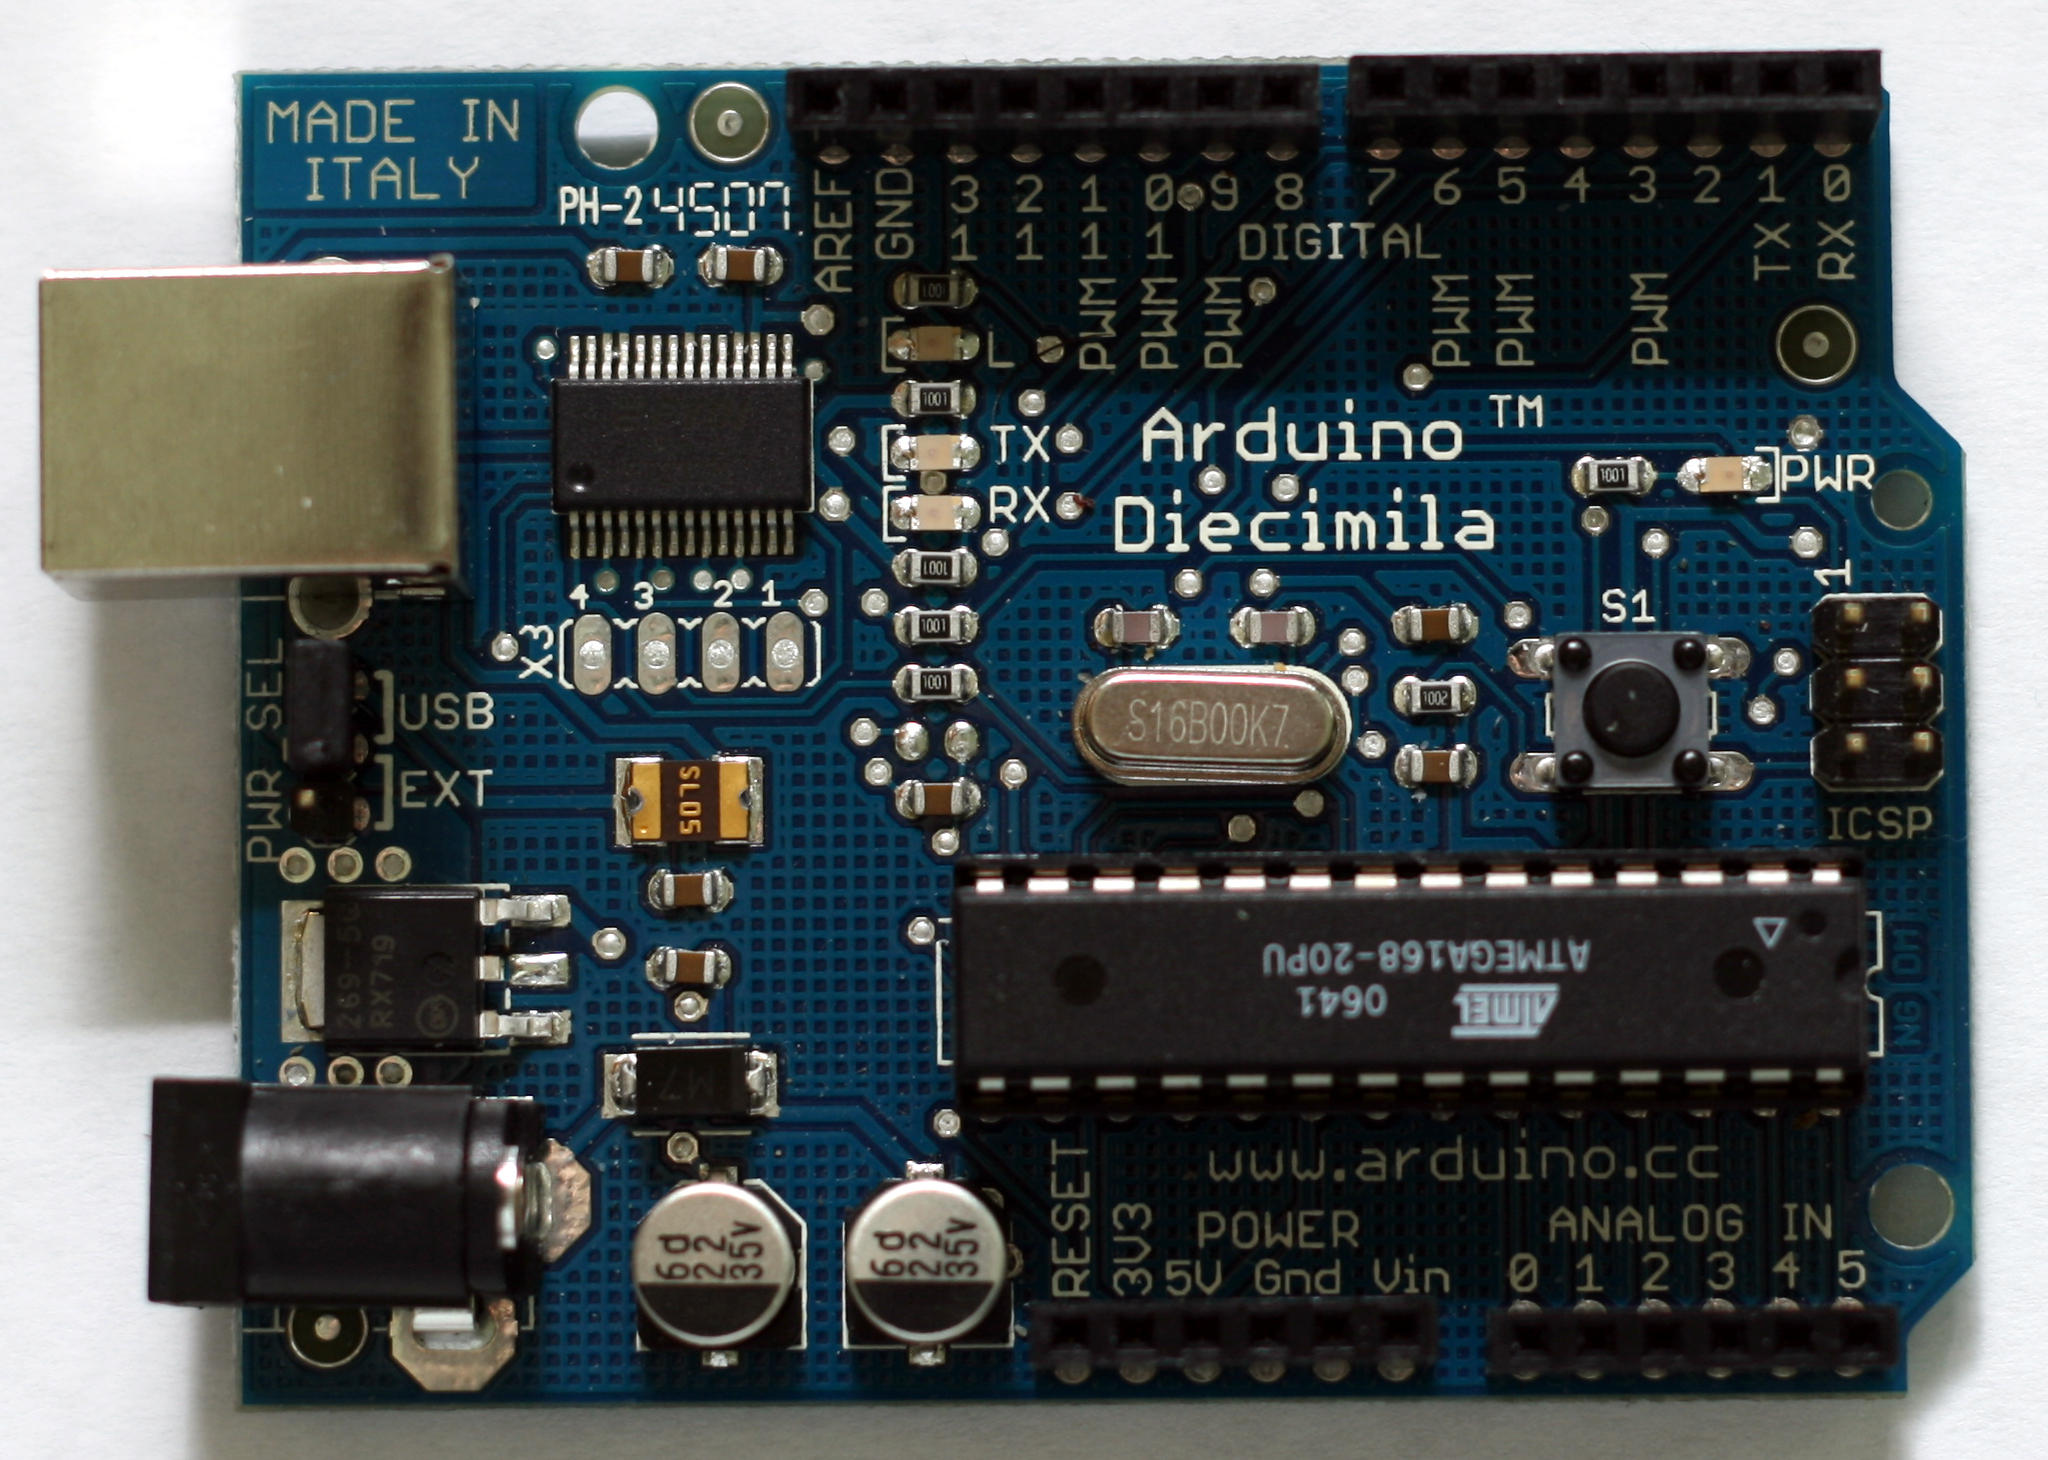
\includegraphics[width=4cm]{Arduino_Diecimila.jpg}};
\end{tikzpicture}
\end{frame}

\subsection{}
\begin{frame}{Open Source věci}
\begin{itemize}
\item 3D tisk získává na popularitě
\item CNC, frézování, řezání laserem \\ (substraktivní) vs. tisk (aditivní)
\item Tisk plastem (horizontální vrstvy, \\ ABS nebo PLA) vs. pryskyřice
\item RepRap stojí 10--20 tisíc korun, \\ částečně zreplikovatelný
\vskip 3ex
\item Repozitář {\em věcí} thingiverse.com:  stáhni CAD soubor a tiskni!
\item Srandičky --- píšťalky, akční figurky, přívěsky, hračky
\item Praktické --- držáky, háčky, kliky, jednoduché nástroje, brýle
\item Součástky --- náhradní díly nebo vlastní projekty
\end{itemize}
\begin{tikzpicture}[remember picture,overlay]
  \node [xshift=-4.25cm,yshift=-6cm,above right] at (current page.north east)
    {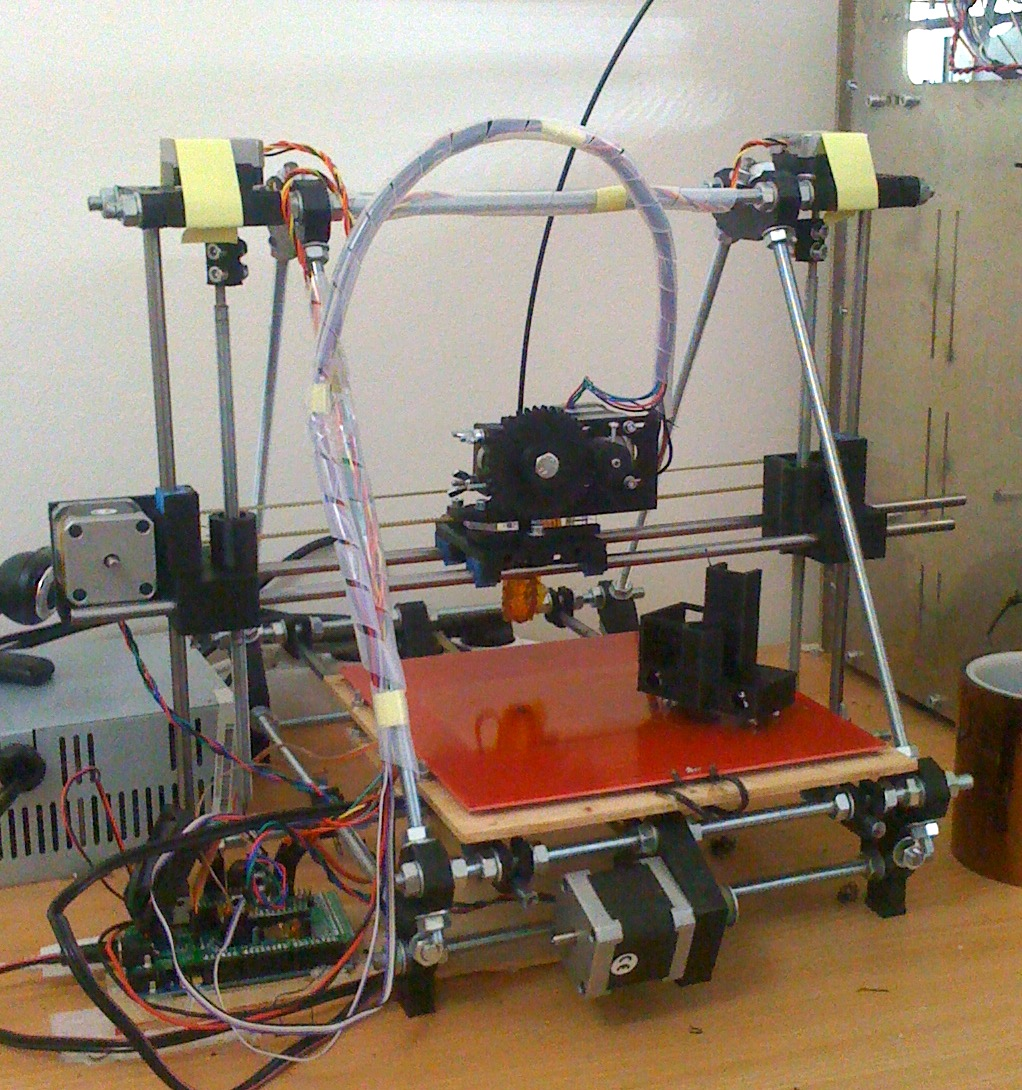
\includegraphics[width=4cm]{Assembled-prusa-mendel.jpg}};
\end{tikzpicture}
\end{frame}


\subsection{}
\begin{frame}{Děkuji za pozornost}
\begin{center}
Příště: Život a údržba otevřených projektů.
\end{center}
\end{frame}

\end{document}
